


% svg debiliškai gaunas, sueis screeshot'as for the moment
% redaguoti galima čia https://demo.bpmn.io/s/start
% originalus failas: processes.bpmn

\begin{landscape}
\section{Procesų aprašymas}
\thispagestyle{empty}
\begin{figure}[H]%[htpb!]
    \centering
    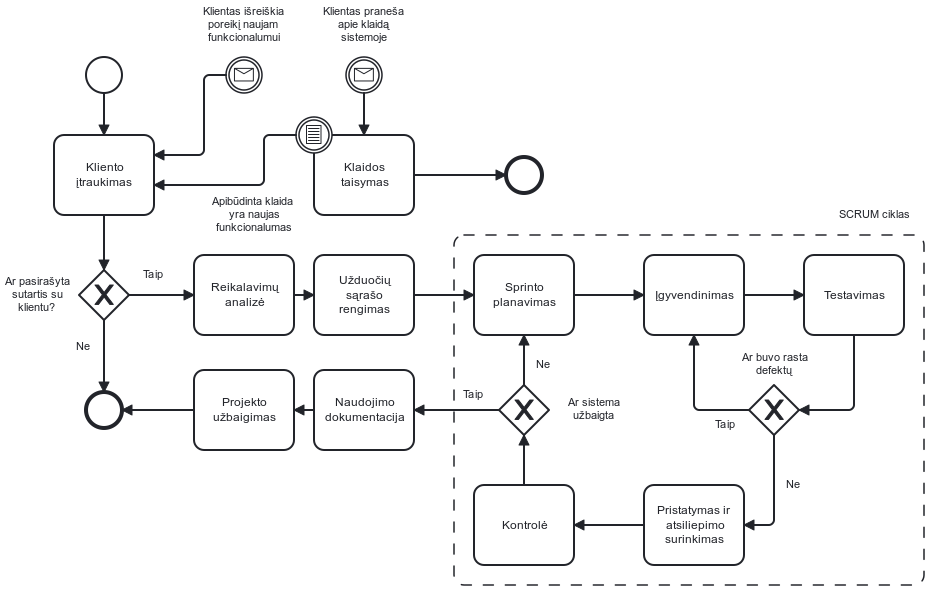
\includegraphics[width=0.9\linewidth]{etc/diagrams/processes.png}
\end{figure}
\end{landscape}

\subsection{\process{EngageClient}} % ARNAS

\begin{figure}[H]%[htpb!]
    \centering
    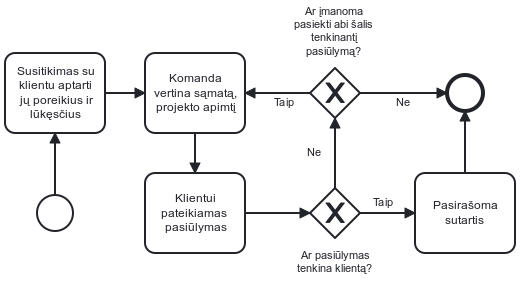
\includegraphics[width=0.75\linewidth]{etc/diagrams/engage-client.png}
\end{figure}

\begin{processTable}{EngageClient}
    \tikslas{Siekiama įvertinti kliento poreikius, rasti kompromisą dėl projekto sąmatos bei apimties ir pasirašyti sutartį}
    \inputs{
        \item \textit{KP}. Kliento poreikiai ir galimybės
        \item \workProd{Experience}
    }
    \outputs{   
        \item \workProd{ResourceEstimates}
        
        \item \workProd{ProjectScope}
        
        \item \workProd{Contract}
    }
    \veiklos{
         \item Projektų vadovas, architektas ir analitikas bendrauja su klientu, aiškinasi jo poreikius sistemai ir vertina kliento galimybes finansuoti tokios sistemos kūrimą. Ši veikla tęsiasi tol, kol įmonės atstovai surenka pakankamai informacijos paruošti klientui pasiūlymą.
    
        \item Projektų vadovas, architektas ir analitikas tarpusavyje įvertina kliento norus ir galimybes ir paruošia sutartį į kurią įeina laiko, kainos ir žmogiškųjų ištekliu sąmata bei nusakoma sistemos apimtis. \label{activity:prepare-deal}

        \item Klientui yra pateikiama sutartis. Jei klientas yra patenkintas sutarties sąlygomis pereinama prie sutarties pasirašymo \textbf{\ref{activity:sign}}. Klientas gali nesutikti su sutarties sąlygomis. Tokiu atveju klientas pateikia naujus poreikius ir dar kartą vykdoma veikla \textbf{\ref{activity:prepare-deal}}. Jei abi šalys nesugeba rasti kompromiso, procesas gali būti nutrauktas ir darbas su klientu netęsiamas.

        \item Pasirašoma sutartis su klientu. \label{activity:sign}
    }
\end{processTable}

\newpage
\subsection{\process{RA}} % DOMANTAS

\begin{processTable}{RA}
    \tikslas{
        Nustatomi funkciniai ir nefunkcinai reikalavimai, kuriuos turi atitikti sistema, atitinkamai suprojektuojama sistema.
    }
    % Surinkti/nustatyti/išvesti? funkcinius ir nefunkcinius reikalavimus
    % Derive technical requirements that the system must meet and design the system accordingly.
    \inputs{
        \item \workProd{ResourceEstimates}
        \item \workProd{ProjectScope}
        \item \workProd{Contract}
    }
    \outputs{
        \item \workProd{FunReq}
        \item \workProd{NonFunReq}
        \item \workProd{HighLevelArch}
        % Architecture
    }
    \veiklos{
        % TODO: pridėt kas atlieka tas veiklas
        \item Pagal sutartį su klietu (\workProdId{Contract}) sąlygas, analistas identifikuoja suinteresuotas šalis ir informacijos šaltinius.
        \item Analistas renka informaciją iš suinteresuotų šalių per interviu ir modeliuoja įmonės
        procesus iš identifikuotų informacijos šaltinių.
        \item Analistas iš surinktos informacijos identifikuoja konkrečius vartotojų poreikius
        % \item Perform analysis of gathered intel, document concrete user needs (\textit{UN}).
        \item Architektas apibrėžia funkcinius (\workProdId{FunReq}) ir nefunkciniai reikalavimus (\workProdId{NonFunReq}) iš identifikuotų vartotojų poreikių; laiko kainos, žmogiškųjų išteklių sąmatos ir projekto apimties  \workProdId{ResourceEstimates}.
        \item Architektas sukuria aukšto lygio sistemos architektūrą (\workProdId{HighLevelArch}) atsižvelgdamas į apibrėžtus funkcinius (\workProdId{FunReq}) ir nefunkcinius reikalavimus (\workProdId{NonFunReq}).
    }
\end{processTable}

\newpage
\subsection{\process{DraftBacklog}} % ARNAS

\begin{processTable}{DraftBacklog}
    \tikslas{Paversti analizės metu išskirtus reikalavimus ir sistemos architektūra į panaudos atvejus ir užduotis iš kurių būtų sudaromas užduočių sąrašas}
    \inputs{
        \item \workProd{FunReq}
        \item \workProd{NonFunReq}
        \item \workProd{HighLevelArch}
    }
    \outputs{
        \item \workProd{Backlog}
    }
    \veiklos{
         \item Architektas kartu su analitiku agreguoja analizės metu surinktus reikalavimus bei aukšto lygio sistemos architektūra į panaudos atvejus ir projekto užduotis. Jie taip pat užtikrina, kad visos projekto užduotys ir panaudos atvejai turėtų detalų aprašymą ir aiškius priėmimo kriterijus. 
    }
\end{processTable}

\newpage
\subsection{\process{ScrumCycle}}

%  ## Domanto klausimai
% 
%  - Jeigu sprinto backlog'e įdedamos klaidos (t.y. klaida yra tiesiog dar vienas task'as sprinto užduočių sąraše), kam tada reikalingas "KL. Klaidos" darbo produktas?

\subsubsection{\process{Refinement}}

\begin{processTable}{Refinement}
    \tikslas{
        Peržiūrėti ir išskaldyti užduotis iš projekto užduočių sąrašo į mažesnes, lengviau valdomas sprinto užduotis, kurias gali atlikti programinės įrangos kūrėjai.
        % Koreguoti prioritetus ir užtiktinti užduočių aiškumą taip, kad užduotys atitiktų tikstus. Nusprendžiama kurios sprinto užduotys bus atliekamos ir kas jas atliks šį sprintą.
    % Review and refine the backlog of tasks by breaking them into smaller, more manageable parts. Adjust priorities and ensure clarity in the tasks to align with the product goals and
    %    ==decide what and who will execute it this sprint==.
    %       DOM_NOTE: mano supratimu čia blogai X
    }
    \inputs{
        \item \workProd{Backlog}
        % \item \textit{PB}. Project backlog
        \item \workProd{SprintReviewDoc}
        % \item ==\textit{SP}. Story points range==
        %   DOM_NOTE: gal blogai, kad šio proceso pirmu atlikimu nėra niekur apibrėžtas SP? 
        (tik nuo antro sprinto)
        \item \workProd{StoryPointRange} (tik nuo antro sprinto)
        
        % \item \textit{SRR}. Sprint review report   
    }
    \outputs{
        \item \workProd{SprintBacklog}
    %     \item \textit{PB}. Project backlog
        \item \workProd{Backlog}
    % \item \textit{SB}. Sprint backlog
    }
    \veiklos{
        \item Projektų vadovas, kuris atsižvelgia į sprinto peržiūros ataskaitą (\workProdId{SprintReviewDoc}), nustato sprinto tikslus. Jei istoriniai praėjusių sprintų duomenys dar neegzistuoja, nes vykdomas pirmasis sprintas, atsižvelgia į projektų užduočių sąrašo (\workProdId{Backlog}) pirminę prioritizaciją.
        \item Visa scrum komanda dalyvauja bendrame susitikime.
        \item Projektų vadovas 1  veikloje įvardintus tikslus pasako komandai. Į tai atsižvelgę komandos nariai (\workProdId{Backlog}) gali keisti užduočių atributą „prioritetas“, taip sudarydami naują užduočių prioriteto eilę.
        \item Jei komandos nariai nusprendžia, kad tam tikra užduotis iš projekto užduočių sąrašo (\workProdId{Backlog})  turi būti išskaidoma į mažesnes, atomiškas užduotis, tai ir yra atliekama. Šios veiklos metu skaidoma užduotis ištrinama, tačiau (\workProdId{Backlog}) sukuriamos kelios smulkesnės užduotys. Šių užduočių prioritetas taip pat gali būti keičiamas.
        \item Komanda kiekvienai sprinto užduočiai įvertina pastangas, kurių reikės jai atlikti, naudojant pasakojimo vienetus, įprastai sekančius Fibonači seką.  Tai atliekama remiantis kelių komandos narių darbine patirtimi ir bendru susitarimu. Tuomet (\workProdId{Backlog}) esančios užduoties atributas „pasakojimo vienetai“ keičiamas į nutartą skaičių.
        \item Projektų vadovas sukuria sprinto užduočių sarašą (\workProdId{SprintBacklog}) atsirinkdamas aukščiausio prioriteto  užduotis iš projekto užduočių sąrašo (\workProdId{Backlog})  taip, kad jų bendra pasakojimo vienetų suma tilptų į pasakojimo vienetų intervalą (\workProdId{StoryPointRange}). Pirmojo sprinto metu, dar neturint pasakojimo vienetų intervalo, parenkama tiek užduočių, kiek komanda bendru nutarimu nusprendžia.
        \item Komandos nariai planuoja, kas atliks kurią sprinto užduotį. Nutarus, sprinto užduočių sąraše (\workProdId{SprintBacklog}) kiekvienos užduoties „atsakingas asmuo“ atributas keičiamas į už užduoties įgyvendinimą atsakingo asmens vardą ir pavardę. 
    }
\end{processTable}

\newpage
\subsubsection{\process{Development}}

\begin{processTable}{Development}
    \tikslas{
         Atlikti sprinto užduočių sąraše išvardytas užduotis.
    }
    \inputs{
        \item \workProd{SprintBacklog}
        \item \workProd{DefectReport}
        \item \workProd{Codebase}
                \item \workProd{TechDoc}
    }
    \outputs{
        \item \workProd{ProductIncrement}
        
        \item \workProd{Codebase}
        
        \item \workProd{TechDoc}
    }
    \veiklos{
        \item Kiekvienas programinės įrangos kūrėjas atlieka jam priskirtą užduotį kaip nurodyta sprinto užduočių saraše (\workProdId{SprintBacklog}) esančių užduočių statuse „atsakingas asmuo“. Laikas, kuris buvo praleistas atliekant 2-6 veiklas pažymimas sprinto užduočių sąraše (\workProdId{SprintBacklog}) esančios užduoties atribute „kūrimo valandos“.
        \item Kiekvienas programinės įrangos kūrėjas rašo kodą, taip papildydami     \workProdId{Codebase}.  
        \item Programinės įrangos kūrėjai rašo funkcijų testus, kurie padengia 70\% kodo eilučių, kad užtikrintų funkcionalumą. Laikoma, kad yra atnaujinamas programinis kodas \workProdId{Codebase}.
        \item Kai kodas ir vienetų testai parašyti, kitas komandos programinės įrangos kūrėjas peržiūri kodą. Jeigu kitas komandos  narys pareikalauja pakeitimų, programinės įrangos kūrėjas turi pakartoti 2-4 veiklas.
        \item Kitam komandos programinės įrangos kūrėjui patvirtinus kodą ir pašalinus visas klaidas, programinės įrangos kūrėjas testavimui parengia
         produkto prieaugį (\workProdId{ProductIncrement})
         atnaujina klaidos aprašymą (\workProdId{DefectReport}). Užduoties būsena sprinto užduočių sąrašę (\workProdId{SprintBacklog}) turi būti atnaujinta, kad atspindėtų, jog užduotį galima testuoti.
        \item Visą reikalingą techninę dokumentaciją (\workProdId{TechDoc}) parašo programinės įrangos kūrėjas.
    }
\end{processTable}

\newpage
\subsubsection{\process{Testing}}

\begin{processTable}{Testing}
    \tikslas{
        Patikrinti, ar produkto prieaugis atitinka kokybės standartus, nepažeidžiant ankstesnių produkto prieaugių.
        % To verify that the product increment meets
        % the defined acceptance criteria % <- RAUDONA
        % and quality standards without breaking something in previous product increments. Testing ensures the product is functional, reliable.
    }
    \inputs{
        \item \workProd{ProductIncrement}
        
        \item \workProd{Codebase}
        
        \item \workProd{TechDoc}
    }
    \outputs{
        \item \workProd{DefectReport}
        \item \workProd{SprintBacklog}
    }
    \veiklos{
         \item Testuotuojai privalo laiką, kurį buvo praleido atliekant 2-6 veiklas susižymėti sprinto užduočių sąraše (\workProdId{SprintBacklog}).
        % NOTE: SUS nėra tarp input'ų
         % \item Testers must log work done in \textbf{2-6} in sprint backlog (\textit{SB}).
         
         \item Testuotuojai ištestuoja produkto prieaugį (\workProdId{ProductIncrement}) pagal \st{priėmimo kriterijus}
         % NOTE: o iš kur parauti priėjimo kriterijai (Acceptance criteria)?
         užduoties, iš sprinto užduočių sarašo (\workProdId{SprintBacklog}), aprašymą.
        % \item Testers review the product increment (\textit{PI}) against acceptance criteria (from \textit{SB}) and requirements, using \textit{DOC} if necessary.

        \item Testuotojai atlieka funkcinių ir nefunkcinių reikalavimų testavimą (t.y. integracijos, greitaveikos, saugumos testavimą) kaip aprašyta užduoties \st{reikalavimuose} aprašyme.
        % \item They perform functional and non-functional testing (e.g. integration, system, performance, and security testing) as per requirements of the tasks.

        \item Testuotojai atlieka (automatizuotą) regresinį testavimą, tam kad užtikrinti, jog produkto prieaugis (\workProdId{ProductIncrement}) neturi neigiamos įtakos esamam funkcionalumui.
        % \item They conduct regression testing (automated) to ensure new changes do not affect existing functionality.

        \item Testuotojai atnaujina klaidų aprašus (\workProdId{DefectReport}), kad jie atspindėtų kokybės būklę.
        % \item They update defect reports (\textit{DR}) % <- RAUDONA
        % to reflect the quality status.

        \item Jei aptinkama klaidų, užduotis grąžinama atgal į kūrimo ciklą, kad išspręsti klaidas. Testuotojas turi pakeisti užduoties būseną, kad sprinto užduočių sąraše (\workProdId{SprintBacklog}) būtų nurodyta, jog ji vėl yra kūrimo stadijoje.
        % \item If defects are found, the task loops back into the development cycle to address the issues. The tester must change the status of the task to reflect that it is back in development in the sprint backlog (\textit{SB}).
    }
\end{processTable}

\newpage
\subsubsection{\process{PartialDelivery}}

\begin{processTable}{PartialDelivery}
    \tikslas{
       Pristatyti suinteresuotosioms šalims produkto prieaugį ir surinkti atsiliepimus.
        % To deliver a  product increment to stakeholders and gather feedback. This process ensures that the product is moving in the right direction and that stakeholder expectations are met
    }

    \inputs{
        \item \workProd{ProductIncrement}
        \item \workProd{DefectReport}
        \item \workProd{Backlog}
    }
    \outputs{
       \item \workProd{Feedback}
    }
    \veiklos{
        % Čia biški pertvarkiau things
        
        % \item Deliver the product increment (\textit{PI}) to stakeholders for initial feedback.
        % \item Present the outcomes of the latest sprint, including the features developed and known issues from \textit{DR}.
        \item Produkto vadovas suinteresuotosioms šalims pristato produkto prieaugį (\workProdId{ProductIncrement}) ir klaidų aprašymus (\workProdId{DefectReport}), tam kad jos pateiktu savo atsiliepimus.

        \item Produkto vadovas išklauso suinteresuotųjų šalių atsiliepimus apie produkto prieaugį (\workProdId{ProductIncrement}) ir jo atitikimą jų poreikiams. Aptaria visus trūkumus, galimus patobulinimus ir pakeitimus projekto užduočių sarašui (\workProdId{Backlog}).
        % \item Collect feedback from stakeholders regarding the delivered increment and its alignment with their needs. Discuss any gaps, potential improvements, and changes to the     \textit{PB}.

        \item Produkto vadovas surašo surinktus atisiliepimus į atsiliepimų registrą (\workProdId{Feedback}).
        % \item Write feedback documentation (\textit{FD}).
    }
\end{processTable}

\newpage
\subsubsection{\process{Control}}

\begin{processTable}{Control}
    \tikslas{
        Peržiūrėti atliktą darbą ir suinteresuotųjų šalių atsiliepimus, kad būtų įvertinta, kaip sekėsi sprintas, laiko valdymą ir suderinti būsimų scrum ciklų patobulinimus.
    }
    \inputs{
        \item \workProd{ProductIncrement}
        \item \workProd{DefectReport}
        \item \workProd{SprintBacklog}
        \item \workProd{ResourceEstimates}
        \item \workProd{StoryPointRange}
        \item \workProd{Feedback}
        \item \workProd{Backlog}
    }
    \outputs{
        \item \workProd{SprintReviewDoc}
        \item \workProd{StoryPointRange}
    }
    \veiklos{
        \item Visi komandos nariai apmąsto sprinto eigą, aptaria, kas pavyko ir su kokiais sunkumais susidūrė. Visi komandos nariai surašo savo komandos atsiliepimus.
        % \item The team reflects on the sprint's progress, discussing what went well and what challenges were encountered.

        \item Projekto vadovas įvertina faktinį užduotims atlikti sugaištą laiką, palygina su pradiniais įverčiais, kad suprastų, kaip komanda valdo laiką, naudodamasis sprinto užduočių sąraše (\workProdId{SprintBacklog}) nurodytomis valandomis ir pradine laiko sąmata (\workProdId{Contract}). Projekto vadovas surašo laiko ataskaitą. % TODO: "Laiko ataskaita" - blogas terminas; sugalvoti kažką geresnio
        % \item The project managed assesses the actual time spent on tasks compared to the initial estimates to understand the team's time management using sprint backlog (\textit{SB}) logged hours and initial time estimates (\textit{EST}).

        \item Remiantis komandos atsiliepimais, laiko ataskaita ir atsiliepimų registru, komanda ir projektų vadovas nustato, kokių pakeitimų reikia kitam sprintui.
        % \item Based on \textbf{1-2} and feedback documentation (\textit{FD}), the project manager and scrum team identifies necessary adjustments for the next sprint.
        Projekto vadovas atlieka projekto užduočių sąrašo (\workProdId{Backlog}) atnaujinimą,
        % NOTE: Bet ar tai tikrai reikia čia atlikti? Gal geriau tai pažymėti sprinto peržiūros ataskaitoj ir td koregavimas atliekamas Sprinto Planavime?? also jeigu keičiama čia, tai reikia pridėti atitinkamai prie input'ų ir output'ų.
        prireikus užduočių prioritetų keitimą ir šių pakeitimų fiksavimą sprinto peržiūros ataskaitoje (\workProdId{SprintReviewDoc}), pasakojimo vienetų intervalo (\workProdId{StoryPointRange}) patikslinimą.
        % This includes updating the project backlog (\textit{PB}), reprioritizing tasks as needed and capturing these changes in the sprint review report (\textit{SRR}), refining the story point range (\textit{SP}).

        \item Jei reikia, projekto vadovas užbaigia projektą - jei daugiau sprintų nebereikia, pereinama prie naudojimo dokumentacijos.
        % NOTE: čia gal nurodyti kokiomis sąlygomis nebereikia kitų sprint'ų?
        % \item The project manager closes project if necessary - if no further sprints are required, they transition to usage documentation.
    }
\end{processTable}

\newpage
\subsection{\process{CreateManual}}

\begin{processTable}{CreateManual}
    \tikslas{Paruošti produkto naudojimo instrukciją, suprantamą naudotojams}
    \inputs{
        \item \workProd{UserNeeds}
        \item \workProd{Backlog}
        \item \workProd{Product}
    }
    \outputs{
            \item \workProd{Manual}
    }
    \veiklos{
        \item Iš užduočių sąrašo (\workProdId{Backlog}) išrenkami panaudos atvejai (Story tipo užduotys) 
        \item Detaliai aprašomi visi žingsniai kiekvienam panaudos atvejui naudojant produktą (\workProdId{Product}). \label{CreateManual/1}
        \item Detaliai aprašomos visos produkto (\workProdId{Product}) funkcijos (t.y. kaip jomis pasinaudoti) \label{CreateManual/2}
        \item Iš \ref{CreateManual/1}. ir \ref{CreateManual/2}. sudaromas struktūrizuotas, vientisas dokumentas - \prodWork{Manual}
        \item Atliekama produkto naudojimo instrukcijos (\workProdId{Manual}) validacija - paruoštas dokumentas peržiūrimas kolegų iš kitų padalinių, įsitikinama, jog instrukcija suprantama pirmą kartą produktą (\workProdId{Product}) naudojantiems žmonėms \label{CreateManual/3}
        \item Kol netenkinamas \ref{CreateManual/3}. punktas, atliekami naudojimo instrukcijos pakeitimai
        }
\end{processTable}

\begin{figure}[!h]
    \centering
    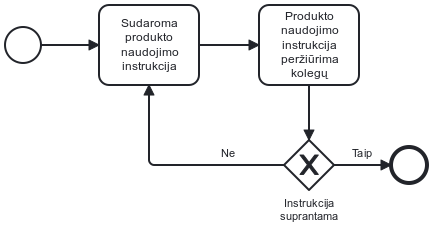
\includegraphics[width=0.75\linewidth]{etc/diagrams/Manual.png}
\end{figure}
% --------------------------------------------------------------------
\newpage
\subsection{\process{CloseProject}}
\begin{processTable}{CloseProject}
    \tikslas{Užbaigti projektą, perduoti paruoštą naudojimui produktą klientams}
    \inputs{
        \item \workProd{Product}
    	\item \workProd{Contract}
    	\item \workProd{Backlog}
    	\item \workProd{TechDoc}
    	\item \workProd{Manual}
    }
    \outputs{
        \item \workProd{Warranty}
        \item \workProd{Experience}
    }
    \veiklos{
         \item Įsitikinama, jog visos užduočių sąraše (\workProdId{Backlog}) numatytos užduotys yra įgyvendintos
        \item Atliekami sutartyje (\workProdId{Contract}) numatyti produkto (\workProdId{Product}) perdavimo klientui darbai
        \item Klientui perduodama \prodWork{Manual}
        \item Klientui perduodama \prodWork{TechDoc}
        \item Sudaroma ir pasirašoma \prodWork{Warranty}, kurioje numatomas garantinio aptarnavimo laikotarpis
    	\item Atliekama vidinė komunikacija apie užbaigtą projektą. Projekto vadovas dalinasi projekto eiga, priimtais kritiniais sprendimais ir rezultatais. Taip kaupiama \prodWork{Experience} 
    	\item Kol nesibaigia sutartyje (\workProdId{Contract}) numatytas adaptacinis laikotarpis, klientams teikiama techninė pagalba
    }
\end{processTable}

\begin{figure}[!h]
    \centering
    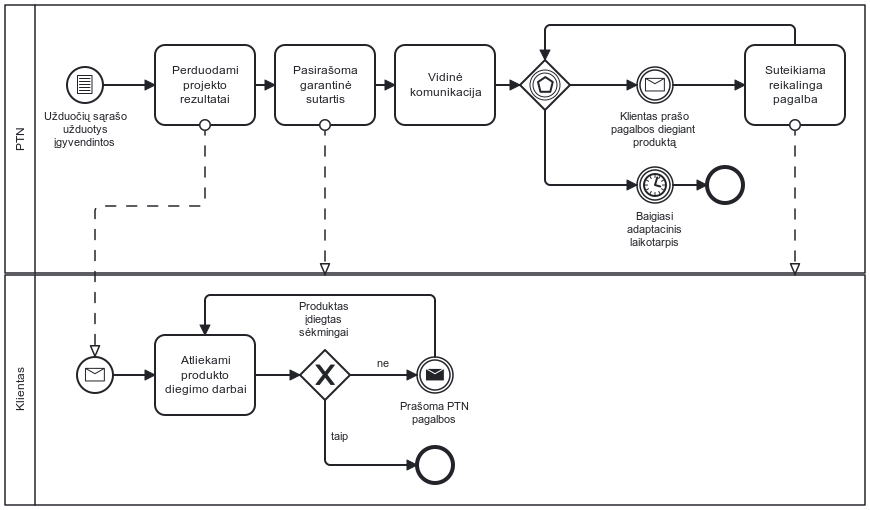
\includegraphics[width=0.8\linewidth]{etc/diagrams/projectClosure.png}
\end{figure}
\newpage

%----------------------------------------


\subsection{\process{BugFix}}
\begin{processTable}{BugFix}
    \tikslas{Ištaisyti ne dėl kliento kaltės kilusias produkto klaidas}
    \inputs{
        \item \workProd{Product}
    	\item \workProd{TechDoc}
    	\item \workProd{Contract}
    	\item \workProd{Warranty}
    	\item \workProd{Ticket}
    	\item \workProd{Manual}
     }
    \outputs{
        \item \workProd{Ticket}
        \item \workProd{Product}
    }
    \veiklos{
        \item Atliekama pirminė užregistruotos klaidos (\workProdId{Ticket}) analizė
	   \item Jei užregistruota klaida (\workProdId{Ticket}):
            \begin{enumerate}[label=\alph*)] 
        		\item kyla dėl produkto (\workProdId{Product}) naudojimo nesilaikant produkto naudojimo instrukcijos (\workProdId{Manual})
        		\item kyla eksploatuojant produktą (\workProdId{Product}) netinkamomis, t.y. neatitinkančiomis techninės dokumentacijos (\workProdId{TechDoc}), sąlygomis
        		\item yra ne klaida, o neegzistuojančio ir sutartyje (\workProdId{Contract}) nenumatyto funkcionalumo įgyvendinimo prašymas
        		\item neatitinka garantino aptarnavimo sutartyje (\workProdId{Warranty}) numatytų sąlygų
        		\item yra užregistruota po garantino aptarnavimo sutartyje (\workProdId{Warranty}) numatyto garantinio laikotarpio
            \end{enumerate}
            tuomet užregistruota klaida (\workProdId{Ticket}) nėra taisoma ir šis procesas (\processId{BugFix}) yra užbaigiamas nevykdant tolesnių veiklų
    	\item Atliekama klaidos kilimo priežasties analizė (root cause analysis)
    	\item Kuo įmanoma greičiau ištaisoma klaida ir sukuriama nauja produkto (\workProdId{Product}) versija
    	\item Nauja produkto (\workProdId{Product}) versija perduodama klientams
    	\item Užregistruota klaida (\workProdId{Ticket}) papildoma su klaidą ištaisančia prdoukto (\workProdId{Product}) versija bei klaidos kilimo priežastimi    
    }
\end{processTable}
\newpage

%----------------------------------------

% \begin{processTable}{PrimaryKey}
%     \tikslas{}
%     \inputs{
%        \item \workProd{Kazkas}
%     }
%     \outputs{
%        \item \workProd{Kazkas}
%     }
%     \veiklos{
%         \item Kazkokia veikla
%     }
% \end{processTable}


%----------------------------------------